\documentclass{article}
\usepackage{../HW}
\numberwithin{table}{section}
\numberwithin{figure}{section}

\title{COMP3711 Assignment 5}
\usetikzlibrary{positioning}
\tikzset{%
every neuron/.style={
    circle,
    draw,
    minimum size=1cm
},
neuron missing/.style={
    draw=none, 
    scale=4,
    text height=0.333cm,
    execute at begin node=\color{black}$\vdots$
},
}


\begin{document}
\maketitle

\begin{section}{Max-Flow and Graph Reliability}
Let $G = (V, E)$ be a directed graph with two specified vertices $s, t \in V$. Assume that $G$ contains at least one $s-t$ path.

A subset of edges $E_0 \subseteq E$ is a separating edge set if, after removing $E'$ from $G$, no $s-t$ path exists.

A subset $V' \subseteq V - fs$, tg of vertices is a separating vertex set if, after    removing $V'$ and all edges connected to $V'$ from $G$, no $s-t$ path exists. If $(s, t) \notin E$, a separating vertex set always exists.

$E'$ is a smallest separating edge set if it contains the smallest number of edges among all separating edge sets. $V'$ is a smallest separating vertex set if it contains the smallest number of vertices among all separating vertex sets.

Note that a smallest separating edge set E' might not be unique. A smallest separating vertex set $V'$ also might not be unique.

In the graph below $\cbracket{(a, f), (d, g), (e, h)}$ is a smallest separating edge set, but there are others as well.  $\cbracket{g,f}$ and $\cbracket{g,a}$ are the only smallest separating vertex sets.

Smallest separating sets are indicators of failure points in a network and are therefore used in studies of network reliability.

In what follows you may use any facts or algorithms taught in class as long as you explicitly reference them (which means including their statement and where in the class or tutorial notes you found them).

Both (a) and (b) should contain 3 parts. Part (i) should describe your algorithm clearly (code is not necessary). Part (ii) should prove its correctness. Part (iii) should derive its running time. Your proof of correctness must contain a section that EXPLICITLY justifies why your output is a smallest separating edge or vertex set.

\begin{enumerate}
    \newpage
    \item Give an $O(|E|^2)$ time algorithm for finding a smallest separating edge
    set for $G$

    \begin{tcolorbox}
        \begin{enumerate}[(i)]
            \item Algorithm for finding smallest separating edge set for $G$.
            
            \begin{itemize}
                \item Assume every edge $e \in E$ has capacity $c_e = 1$, run Ford-Fulkerson Algorithm on $G = (V, E)$ to find a path with maximum flow $P$. The flow network is an edge disjoint path $s-t$.
                \item Let $G'$ as the residual graph from running Ford-Fulkerson algorithm and  $E_1, \dots, E_n$ as edge disjoint $s-t$ paths. 
                \item For each edge $e$ in  $E_i$, check if $e$ is in a cycle in the residual graph $G'$ by running DFS and finding any back edge. 
                \item If yes, check the next edge. If not, $e$ is a separating edge for $E_i$, then reverse the path $E_i$ on the residual graph $G'$, and remove the edge $e$. 
                \item Append $e$ to the answer and proceed with $E_{i+1}$ until all disjoint edge paths are checked.
            \end{itemize}

            \item Proof of correctness:
            
            \textbf{Lemma:} An edge in a cycle in the residual graph is not a separating edge.

            Proof: We can reverse the direction of the edges in the cycle, and we will get another disjoint path. Therefore the flow can be redirected to another edge if we disconnect this edge, and will not separate the graph.

            \textbf{Lemma:} A separating edge must exist in a disjoint path. 

            Proof: We define a separating edge as an edge in a path that is not in a cycle. By contradiction, if there no edge that is not in a cycle within a path, then it implies that there is a path connecting $s-t$, which implies that the Ford-Flukerson algorithm is not completed.

            \textbf{Lemma:} The number of edge disjoint path is equal to the number of minimum separating edge.

            Proof. From the previous lemma, then there is at least 1 edge in an edge disjoint path that can separate the path. To completely separate all paths, then we can choose any separating edge from the edge disjoint paths. Therefore, the total number of edge disjoint path must be the same as the minimum separating edge by choosing exactly one edge from each edge disjoint path.

            \item Running time analysis:
            
            \begin{itemize}
                \item Running time of Ford-Flukerson: $O(\#iter \times |E|)$, where $\max \#iter = |f^*| = O(|E|)$. Therefore, running time of Ford-Flukerson: $O(|E|^2)$
                \item Running time of cycle detection for a single edge: $O(|E|)$. Running time of cycle detection for all edges: $O(|E|^2)$.
            \end{itemize}
            
            Therefore the total running time is: $O(|E|^2)$.
        \end{enumerate}
    \end{tcolorbox}

    \newpage
    \item Assume $(s, t) \in E$. Give an $O(|V||E|)$ time algorithm for finding a smallest separating vertex set for $G$.
    
    \begin{tcolorbox}
        \begin{enumerate}[(i)]
            \item Algorithm for finding smallest separating vertices set for $G$.
            
            This is simply modifying the algorithm of part (a). The idea is to substitute all vertices $v \in V$ with two vertices $v_l, v_r$ (except $s$ and $t$) connected by an `internal edge' $(v_l, v_r) \in E_1'$, and the let the edge $(u, v) \in E$ to be `external edge' $(u_r, w_l) \in E_2'$. 

            Then run the algorithm in part (a) to find the `minimum separating internal edge', with a modification that this algorithm must find internal edges only.

            \item Proof of correctness:
            
            \textbf{Lemma:} Removing the internal edge of $v$ has the same impact to the graph connectivity as removing all edges connected to $v$. 

            Proof. If the internal edge of $v$ is disconnected, then there is no flow passing the external edge of $v$. It is the same as removing all the external edge of $v$.

            By definition $v$ is a separaing vertex if after removing all (external) edges connected to $v$, no $s-t$ path exists.

            By assuming the correctness of the algorithm in (a), then the smallest separating vertex set is the same as the same as the smallest separating internal edge set from the result of algorithm (a).

            \item Running time analysis:
            
            Editing the graph takes $O(|V|+|E|)$, and running the Ford Fulkerson algorithm takes $O(|V|(||V|+|E|))$ as well. 
            Now after the modification, we only check the internal edge. The number of internal edge is $|V|$, and the cycle detection takes $O(|E|+|V|)$. Therefore the total running time is $O(|V| \times (|V|+|E|)) = O(|V| |E|)$.
        \end{enumerate}
    \end{tcolorbox}
\end{enumerate}

\end{section}

\newpage
\begin{section}{Max Flow}
Modified from Kleinberg and Tardos, Chapter 7, Exercise 16.

Google makes money by selling targeted advertising, using what it knows about you.

When you do a search Google shows you an ad. A specific ad is shown to you because an advertiser requested that this ad be shown to a person in a demographic group to which you belong.

In this problem you will design an algorithm to decide whether Google can satisfy a collection of targeted requests made by advertisers.

\begin{itemize}
    \item $\mathbf{U}$ is the universe of people currently online. $U = \cbracket{p_1, \dots , p_n}$.
    \item $\mathbf{X}_i, j = 1 \dots m$ are subsets of $U$ that \textit{cover} $U$, i.e., $\forall j, \mathbf{X}_j \subseteq U$ and
    $S_j \mathbf{X}_j = U$.
    The $\mathbf{X}_i$ are demographic groups. For example, $\mathbf{X}_1$ might be all middleaged professors with two children. The $\mathbf{X}_i$ are defined by inputs $D_{i,j}$
    for $1 \leq i \leq n, 1 \leq j \leq m$.
    \begin{align*}
        D &=
        \begin{cases}
            1 & \text{If $p_i \in \mathbf{X}_j$, i.e., person $p_i$ in Demographic Group $j$,} \\
            0 & \text{If $p_i \notin j$}
        \end{cases}
    \end{align*}
    \item There are $r$ Advertisers (companies). Advertiser $k$ wants its ads shown to at least $P_k$ people.
    \item Furthermore, each advertiser only wants to show ads to people within specific targeted collections of demographic groups. We denote these constraints as follows. The collections are defined by variables $Y_{j,k} \in \cbracket{0,1}, 1 \leq j \leq m, 1 \leq k \leq r$. Set
    \begin{align*}
        \mathbf{Z}_k = \bigcup_{\cbracket{j:Y_{j,k}=1}} \mathbf{X}_j
    \end{align*}
    Advertiser $k$ wants its advertisements only to be shown to people in $\mathbf{Z}_k$.
    \item Each Advertiser provides Google with one advertisement. Each person can only be shown one advertisement, i.e., from one Advertiser.
\end{itemize}

The inputs to the problem are the values of $D_{i,j}$, $Y_{j,k}$, and $P_k$. The problem is now to find out if Google can devise an advertising policy satisfying all of the advertisers requests.

That is, can Google show each person at most one ad so that exactly $P_k$ people see the ad from Advertiser k and these $P_k$ people are all in the set Zk.

Your algorithm should run in $O ((\sum_k P_k) mn)$ time.

\begin{enumerate}[(a)]
    \item Design an $O ((\sum_k P_k) mn)$ time algorithm for deciding if it is possible for Google to satisfy all of the requests.
    
    Your algorithm does not need to be in pseudocode. It does need to be understandable, though. Do not write it as one paragraph. 
    
    Instead, present the algorithm in numbered point notation, putting each step in a different numbered point.

    If satisfaction is possible, you should output which advertiser’s ad each person is shown (or if a person is not shown an ad). That is, you should output $n$ pairs $(i, k)$ denoting that $p_i$ is shown advertisement $k$ (where $k = 0$ if $p_i$ is not shown any ad).

    Your algorithm may use any algorithm shown in class as a subroutine.
    
    \begin{tcolorbox}[breakable]
        The idea is to calculate the max flow from the network for each $k$. The algorithm can be described as follows:
        \begin{itemize}
            \item First check if $r > n$, if so, then it wont be possible to satisfy all request. If not, proceed to the next step.
            
            \item Create a flow network with these `layers'. Note that all edges are directed to the next layer.
            
            \begin{figure}[H]
                \centering
                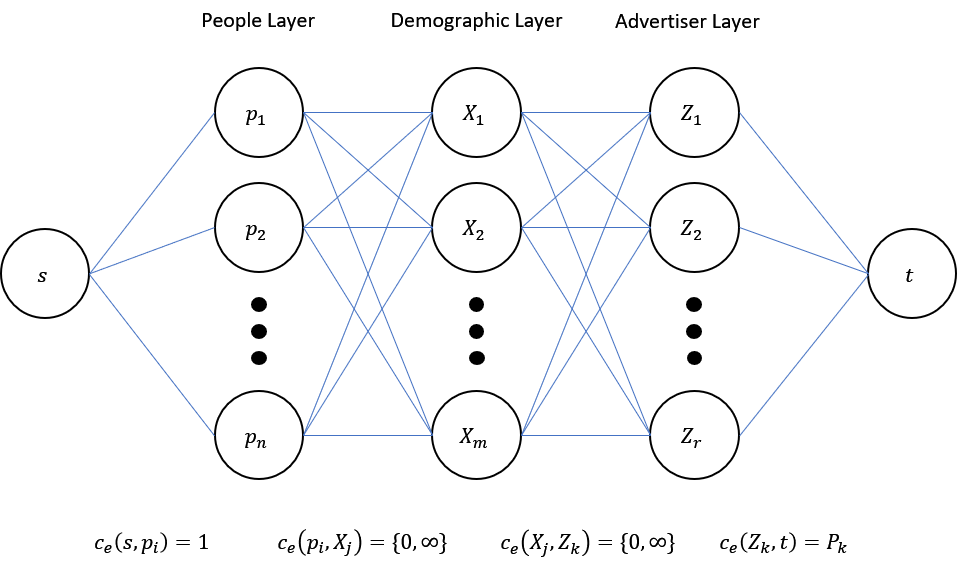
\includegraphics[width=0.9\linewidth]{figures/p2/1.png}
            \end{figure}

            The first layer is the People Layers, connected with the source node $s$ by edges with capacity of one. 
            \begin{align*}
                c_e(s, p_{i}) = 1
            \end{align*}

            The second layer is the Demographic Group Layer, representing the demographic group $X_1, \dots, X_m$. It is connected with previous layer with:
            \begin{align*}
                c_e(p_{i}, X_j) = \begin{cases}
                    0 & \text{if $D_{ij} = 0$} \\
                    \infty & \text{if $D_{ij} = 1$} \\
                \end{cases}
            \end{align*}

            The third layer is the Advertiser Layer, representing the advertiser group $Z_k$ which advertisement $k$ will be shown to. It is connected with previous layer with:
            \begin{align*}
                c_e(X_j, Z_k) = \begin{cases}
                    0 & \text{if $Y_{jk} = 0$} \\
                    \infty & \text{if $Y_{jk} = 1$} \\
                \end{cases}
            \end{align*}

            The target node $t$ is connected with previous layer $Z$ with:
            \begin{align*}
                c_e(Z_k, t) = P_k
            \end{align*}

            \item Then run Ford-Fulkerson algorithm to find the max flow in the flow graph for each advertisement $k$
            
            \item Compare the flow for each $Z_k$ with $P_k$. If $Z_k \geq P_k$ for all $k$, then the request is fulfilled, otherwise the request is not fulfilled.  
            
            \item If fulfilled, then for each $p_i$ in the flow network graph, reduce flow in the path $s-p_i-X_j-Z-k-t$ by $1$ and output $(i, k)$. If such path does not exists, output $(i, 0)$ as the problem description requires. 
        \end{itemize}
    \end{tcolorbox}
    
    \item Explain why your algorithm is correct.
    
    If your explanation invoves an ``if and only if" statement, then you need to explicitly prove the correctness of both directions of the ``if and only if" statement (as in the proof of correctness of the solution of the maximum distinct paths problem taught in class).

    \begin{tcolorbox}
        \textbf{Lemma:} Each person can receive at most one advertisement. 

        Each $p_i$ is connected with the source node by an edge with capacity of 1. The residual graph represents the type of advertisement a person can receive. Then it can only provide at most one flow to the network and receive at most one flow in the residual graph. Therefore, each person can receive at most one advertisement.

        \textbf{Lemma:} The flow network will provide each advertiser with maximum of $P_k$. The maximum flow is $\sum_k P_k$

        Proof. It is limited by the edge conencting $(Z_k, t)$.

        \textbf{Lemma:} If and only if the flow network can provide $\sum_k P_k$ flow, then all advertising request is satisfied.

        Proof. If the node on the Advertisement Layer $Z_j$ provides $P_k$ flow, then the advertising request is fulfilled. If all nodes in the advertiser layer provides $\sum_k P_k$ in total, then all request is satisfied. 
        
        Conversely, if all advertising request is satisfied, then by definition the each advertiser must receive at least more than $P_k$. As the number of advertisement is represented by the flow in the flow network, then all advertising is satisfied if the flow is larger than or equal to $P_k$. But from previous lemma, the flow is limited by $P_k$. Therefore, the total flow must be exactly equal to $P_k$.

        \textbf{Final Proof:} Each person can only receive one advertising by previous lemma and the all advertising request is satisfied when the total flow is exactly $P_k$. The grouping of people to the demographic group and advertisement group is correct trivially. 

        By running Ford-Fulkerson algorithm, it will find the maximum flow in the graph. 
        If the flow is less than $\sum_k P_k$, then there exist some advertiser whose request is not satisfied.
        By previous lemma, all request is satisfied if and only if the maximum flow is $\sum_k P_k$.
    \end{tcolorbox}

    \item Explain why your algorithm runs in $O ((\sum_k P_k) mn)$ time.
    \begin{tcolorbox}
        The running time for running Ford Flukerson Algorithm is $O(\#iter \times |E|)$. By description in the lecture $\#iter = O(|f^*|)$ where $|f^*|$ is the max flow. The max flow is given by $O(\sum_k P_k)$, and the number of edges is given by $|E| = n + nm + mr + r$. But from the first checking from algorithm, we can assume $n > r$, therefore $|E| < n + nm +nm + n = O(mn)$. 
        
        Therefore the total running time is $O((\sum_k P_k) nm)$.
    \end{tcolorbox}
\end{enumerate}
\end{section}

\newpage
\begin{section}{All-Pairs Shortest Paths}
Solve the all-pairs shortest path problem on the given directed graph $G$. $W$ is the weighted adjacency matrix of $G$.

\begin{align*}
    W = \begin{pmatrix}
        & A & B & C & D & E & F & G & H \\
        A & 0 & 4 & 8 & 15 & \infty & \infty & \infty & \infty \\
        B & \infty & 0 & \infty & \infty & 9 & \infty & \infty & \infty \\
        C & \infty & 12 & 0 & \infty & -6 & 8 & \infty & \infty \\
        D & \infty & \infty & 11 & 0 & \infty & -4 & 2 & \infty \\
        E & \infty & \infty & \infty & \infty & 0 & 13 & \infty & 5 \\
        F & \infty & \infty & \infty & \infty & \infty & 0 & 10 & 2 \\
        G & \infty & \infty & \infty & \infty & \infty & \infty & 0 & 9 \\
        H & -5 & \infty & \infty & \infty & \infty & \infty & \infty & 0 \\
    \end{pmatrix}
\end{align*}
\begin{enumerate}[(A)]
    \item Apply the 2nd dynamic programming solution on Page 37, 17 Shortest Path,
    using the recurrence of $d_{ij}^{(2S)} = \min_{1 \leq k \leq n} \cbracket{d_{ik}^{(S)} + d_{kj}^{(S)}}$.

    To answer this question, fill in the following $D^{(S)}$ matrices for each
    step. \textit{Note that} $D^{(1)} = W$.

    \begin{tcolorbox}
    \begin{multicols}{2}
            \resizebox{.9\linewidth}{!}{$
            D^{(1)} = \begin{pmatrix}
                & A & B & C & D & E & F & G & H \\
                A & 0 & 4 & 8 & 15 & \infty & \infty & \infty & \infty \\
                B & \infty & 0 & \infty & \infty & 9 & \infty & \infty & \infty \\
                C & \infty & 12 & 0 & \infty & -6 & 8 & \infty & \infty \\
                D & \infty & \infty & 11 & 0 & \infty & -4 & 2 & \infty \\
                E & \infty & \infty & \infty & \infty & 0 & 13 & \infty & 5 \\
                F & \infty & \infty & \infty & \infty & \infty & 0 & 10 & 2 \\
                G & \infty & \infty & \infty & \infty & \infty & \infty & 0 & 9 \\
                H & -5 & \infty & \infty & \infty & \infty & \infty & \infty & 0 \\
            \end{pmatrix}
            $}

            \resizebox{.9\linewidth}{!}{$
            D^{(2)} = \begin{pmatrix}
                & A & B & C & D & E & F & G & H \\
                A & 0 & 4 & 8 & 15 & 2 & 11 & 17 & \infty \\
                B & \infty & 0 & \infty & \infty & 9 & 22 & \infty & 14 \\
                C & \infty & 12 & 0 & \infty & -6 & 7 & 18 & -1 \\
                D & \infty & 23 & 11 & 0 & 5 & -4 & 2 & -2 \\
                E & 0 & \infty & \infty & \infty & 0 & 13 & 23 & 5 \\
                F & -3 & \infty & \infty & \infty & \infty & 0 & 10 & 2 \\
                G & 4 & \infty & \infty & \infty & \infty & \infty & 0 & 9 \\
                H & -5 & -1 & 3 & 10 & \infty & \infty & \infty & 0 \\
                \end{pmatrix}
            $}

            \resizebox{.9\linewidth}{!}{$
            D^{(4)} = \begin{pmatrix}
                & A & B & C & D & E & F & G & H \\
                A & 0 & 4 & 8 & 15 & 2 & 11 & 17 & 7 \\
                B & 9 & 0 & 17 & 24 & 9 & 22 & 32 & 14 \\
                C & -6 & -2 & 0 & 9 & -6 & 7 & 17 & -1 \\
                D & -7 & -3 & 1 & 0 & 5 & -4 & 2 & -2 \\
                E & 0 & 4 & 8 & 15 & 0 & 11 & 17 & 5 \\
                F & -3 & 1 & 5 & 12 & -1 & 0 & 10 & 2 \\
                G & 4 & 8 & 12 & 19 & 6 & 15 & 0 & 9 \\
                H & -5 & -1 & 3 & 10 & -3 & 6 & 12 & 0 \\
                \end{pmatrix}
            $}

            \resizebox{.9\linewidth}{!}{$
            D^{(8)} = \begin{pmatrix}
                & A & B & C & D & E & F & G & H \\
                A & 0 & 4 & 8 & 15 & 2 & 11 & 17 & 7 \\
                B & 9 & 0 & 17 & 24 & 9 & 20 & 26 & 14 \\
                C & -6 & -2 & 0 & 9 & -6 & 5 & 11 & -1 \\
                D & -7 & -3 & 1 & 0 & -5 & -4 & 2 & -2 \\
                E & 0 & 4 & 8 & 15 & 0 & 11 & 17 & 5 \\
                F & -3 & 1 & 5 & 12 & -1 & 0 & 10 & 2 \\
                G & 4 & 8 & 12 & 19 & 6 & 15 & 0 & 9 \\
                H & -5 & -1 & 3 & 10 & -3 & 6 & 12 & 0 \\
                \end{pmatrix}
            $}

        \end{multicols}
    \end{tcolorbox}

    \newpage
    \item Apply the Floyd-Warshall algorithm on Page 45, 17 Shortest Path,using
    the recurrence $d_{ij}^{(2S)} = \min \cbracket{d_{ik}^{(k-1)}, d_{ik}^{(k-1)} + d_{kj}^{(k-1)}}$.

    To answer this question, fill in the $D^{(k)}$ matrices for each step. \textit{Note
    that} $D^{(0)} = W$.

    \begin{tcolorbox}
    \begin{multicols}{2}
            \resizebox{.9\linewidth}{!}{$
            D^{(1)} = \begin{pmatrix}
                & A & B & C & D & E & F & G & H \\
                A & 0 & 4 & 8 & 15 & \infty & \infty & \infty & \infty \\
                B & \infty & 0 & \infty & \infty & 9 & \infty & \infty & \infty \\
                C & \infty & 12 & 0 & \infty & -6 & 8 & \infty & \infty \\
                D & \infty & \infty & 11 & 0 & \infty & -4 & 2 & \infty \\
                E & \infty & \infty & \infty & \infty & 0 & 13 & \infty & 5 \\
                F & \infty & \infty & \infty & \infty & \infty & 0 & 10 & 2 \\
                G & \infty & \infty & \infty & \infty & \infty & \infty & 0 & 9 \\
                H & -5 & -1 & 3 & 10 & \infty & \infty & \infty & 0 \\
                \end{pmatrix}
            $}

            \resizebox{.9\linewidth}{!}{$
            D^{(2)} = \begin{pmatrix}
                & A & B & C & D & E & F & G & H \\
                A & 0 & 4 & 8 & 15 & 13 & \infty & \infty & \infty \\
                B & \infty & 0 & \infty & \infty & 9 & \infty & \infty & \infty \\
                C & \infty & 12 & 0 & \infty & -6 & 8 & \infty & \infty \\
                D & \infty & \infty & 11 & 0 & \infty & -4 & 2 & \infty \\
                E & \infty & \infty & \infty & \infty & 0 & 13 & \infty & 5 \\
                F & \infty & \infty & \infty & \infty & \infty & 0 & 10 & 2 \\
                G & \infty & \infty & \infty & \infty & \infty & \infty & 0 & 9 \\
                H & -5 & -1 & 3 & 10 & 8 & \infty & \infty & 0 \\
                \end{pmatrix}
            $}

            \resizebox{.9\linewidth}{!}{$
            D^{(3)} = \begin{pmatrix}
                & A & B & C & D & E & F & G & H \\
                A & 0 & 4 & 8 & 15 & 2 & 16 & \infty & \infty \\
                B & \infty & 0 & \infty & \infty & 9 & \infty & \infty & \infty \\
                C & \infty & 12 & 0 & \infty & -6 & 8 & \infty & \infty \\
                D & \infty & 23 & 11 & 0 & 5 & -4 & 2 & \infty \\
                E & \infty & \infty & \infty & \infty & 0 & 13 & \infty & 5 \\
                F & \infty & \infty & \infty & \infty & \infty & 0 & 10 & 2 \\
                G & \infty & \infty & \infty & \infty & \infty & \infty & 0 & 9 \\
                H & -5 & -1 & 3 & 10 & -3 & 11 & \infty & 0 \\
                \end{pmatrix}
            $}

            \resizebox{.9\linewidth}{!}{$
            D^{(4)} = \begin{pmatrix}
                & A & B & C & D & E & F & G & H \\
                A & 0 & 4 & 8 & 15 & 2 & 11 & 17 & \infty \\
                B & \infty & 0 & \infty & \infty & 9 & \infty & \infty & \infty \\
                C & \infty & 12 & 0 & \infty & -6 & 8 & \infty & \infty \\
                D & \infty & 23 & 11 & 0 & 5 & -4 & 2 & \infty \\
                E & \infty & \infty & \infty & \infty & 0 & 13 & \infty & 5 \\
                F & \infty & \infty & \infty & \infty & \infty & 0 & 10 & 2 \\
                G & \infty & \infty & \infty & \infty & \infty & \infty & 0 & 9 \\
                H & -5 & -1 & 3 & 10 & -3 & 6 & 12 & 0 \\
                \end{pmatrix}
            $}
        
            \resizebox{.9\linewidth}{!}{$
            D^{(5)} = \begin{pmatrix}
                & A & B & C & D & E & F & G & H \\
                A & 0 & 4 & 8 & 15 & 2 & 11 & 17 & 7 \\
                B & \infty & 0 & \infty & \infty & 9 & 22 & \infty & 14 \\
                C & \infty & 12 & 0 & \infty & -6 & 7 & \infty & -1 \\
                D & \infty & 23 & 11 & 0 & 5 & -4 & 2 & 10 \\
                E & \infty & \infty & \infty & \infty & 0 & 13 & \infty & 5 \\
                F & \infty & \infty & \infty & \infty & \infty & 0 & 10 & 2 \\
                G & \infty & \infty & \infty & \infty & \infty & \infty & 0 & 9 \\
                H & -5 & -1 & 3 & 10 & -3 & 6 & 12 & 0 \\
                \end{pmatrix}
            $}

            \resizebox{.9\linewidth}{!}{$
            D^{(6)} = \begin{pmatrix}
                & A & B & C & D & E & F & G & H \\
                A & 0 & 4 & 8 & 15 & 2 & 11 & 17 & 7 \\
                B & \infty & 0 & \infty & \infty & 9 & 22 & 32 & 14 \\
                C & \infty & 12 & 0 & \infty & -6 & 7 & 17 & -1 \\
                D & \infty & 23 & 11 & 0 & 5 & -4 & 2 & -2 \\
                E & \infty & \infty & \infty & \infty & 0 & 13 & 23 & 5 \\
                F & \infty & \infty & \infty & \infty & \infty & 0 & 10 & 2 \\
                G & \infty & \infty & \infty & \infty & \infty & \infty & 0 & 9 \\
                H & -5 & -1 & 3 & 10 & -3 & 6 & 12 & 0 \\
                \end{pmatrix}
            $}

            \resizebox{.9\linewidth}{!}{$
            D^{(7)} = \begin{pmatrix}
                & A & B & C & D & E & F & G & H \\
                A & 0 & 4 & 8 & 15 & 2 & 11 & 17 & 7 \\
                B & \infty & 0 & \infty & \infty & 9 & 22 & 32 & 14 \\
                C & \infty & 12 & 0 & \infty & -6 & 7 & 17 & -1 \\
                D & \infty & 23 & 11 & 0 & 5 & -4 & 2 & -2 \\
                E & \infty & \infty & \infty & \infty & 0 & 13 & 23 & 5 \\
                F & \infty & \infty & \infty & \infty & \infty & 0 & 10 & 2 \\
                G & \infty & \infty & \infty & \infty & \infty & \infty & 0 & 9 \\
                H & -5 & -1 & 3 & 10 & -3 & 6 & 12 & 0 \\
                \end{pmatrix}
            $}

            \resizebox{.9\linewidth}{!}{$
            D^{(8)} = \begin{pmatrix}
                & A & B & C & D & E & F & G & H \\
                A & 0 & 4 & 8 & 15 & 2 & 11 & 17 & 7 \\
                B & 9 & 0 & 17 & 24 & 9 & 20 & 26 & 14 \\
                C & -6 & -2 & 0 & 9 & -6 & 5 & 11 & -1 \\
                D & -7 & -3 & 1 & 0 & -5 & -4 & 2 & -2 \\
                E & 0 & 4 & 8 & 15 & 0 & 11 & 17 & 5 \\
                F & -3 & 1 & 5 & 12 & -1 & 0 & 10 & 2 \\
                G & 4 & 8 & 12 & 19 & 6 & 15 & 0 & 9 \\
                H & -5 & -1 & 3 & 10 & -3 & 6 & 12 & 0 \\
                \end{pmatrix}
            $}

        \end{multicols}
    \end{tcolorbox}
\end{enumerate}
\end{section}

\newpage
\begin{section}{Maximum Bipartite Matching}
    Given a matching M (edges highlighted in red) on a bipartite graph $G$ below.

Please draw the flow corresponding to $M$ in the flow network of $G$. To do that, please specify the flow value on each edge in the template below, in the format of $f(e)/c(e)$. Note that $c(e)$ is already given.
\begin{figure}[H]
    \centering
    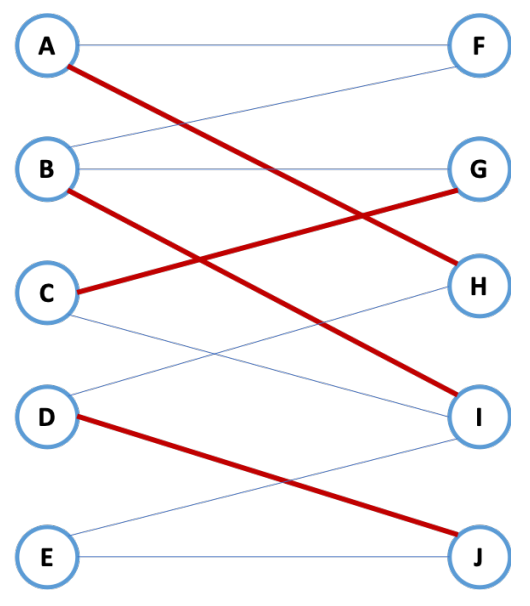
\includegraphics[width=0.4\linewidth]{figures/p4/1.png}
\end{figure}
\begin{enumerate}[(A)]
    \item Please draw the flow corresponding to $M$ in the flow network of $G$. To do that, please specify the flow value on each edge in the template below, in the format of $f(e)/c(e)$. Note that $c(e)$ is already given.
    
    \begin{tcolorbox}
        \begin{figure}[H]
            \centering
            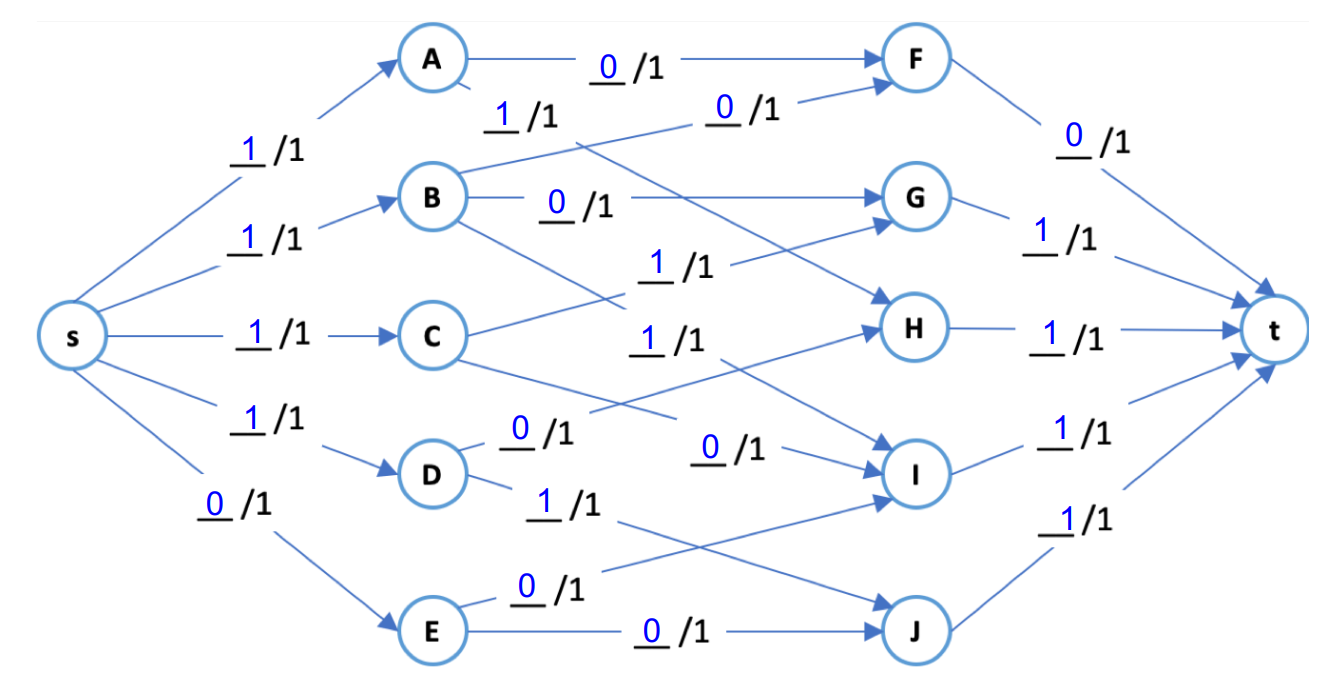
\includegraphics[width=\linewidth]{figures/p4/2.png}
            \caption{Flow network of $G$}
        \end{figure}
    \end{tcolorbox}

    \item Please draw the residual graph corresponding to $M$ on the template
    below. Note that you only need to specify the direction of the edges
    (omitting the residual edge capacities $c_f(e)$, as they are all $1$).

    \begin{tcolorbox}
        \begin{figure}[H]
            \centering
            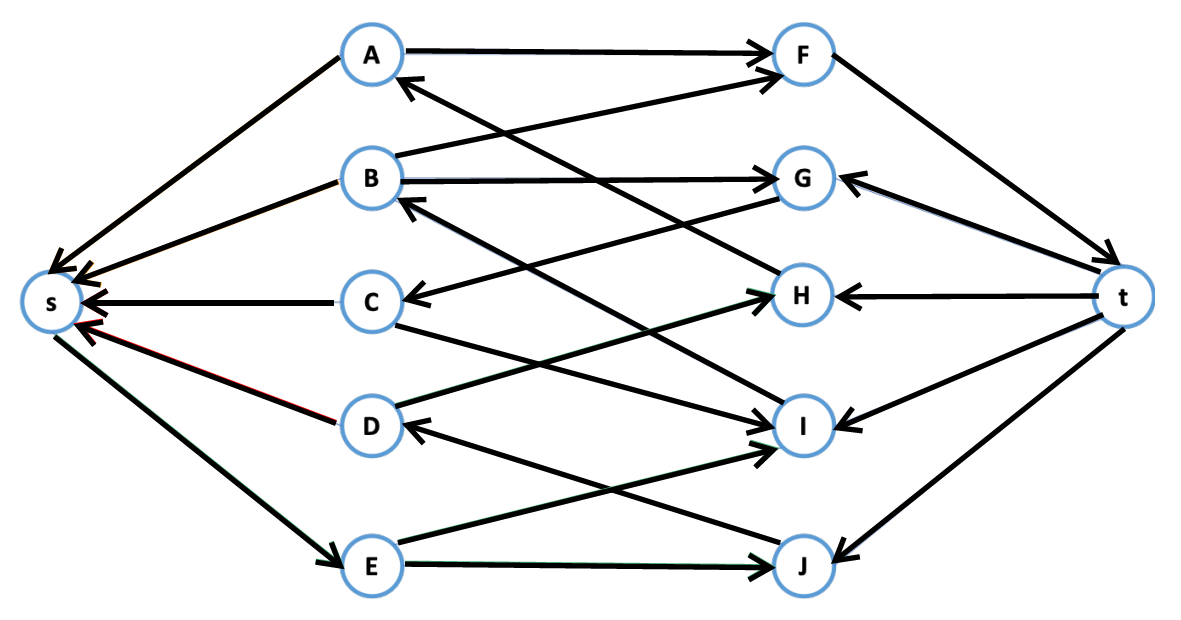
\includegraphics[width=\linewidth]{figures/p4/3.png}
            \caption{Residual graph of $G$} 
        \end{figure}
    \end{tcolorbox}

    \item Is $M$ a maximum bipartite matching of $G$?
    
    If yes, specify the corresponding min $S - T$ cut in the residual graph you have drawn in (B) by highlighting all the nodes in S. 
    
    If no, find an $s - t$ path $P$ in the residual graph you have drawn in (B) by highlighting all the edges in $P$. Then provide the resulting matching $M'$ by highlighting the selected edges in $G$ using the following template. 

    \begin{tcolorbox}[breakable]
        No, $M$ is not a maximum bipartite of $G$, as there is a path $P$ in the residual graph connecting $s-t$. 
        \begin{figure}[H]
            \centering
            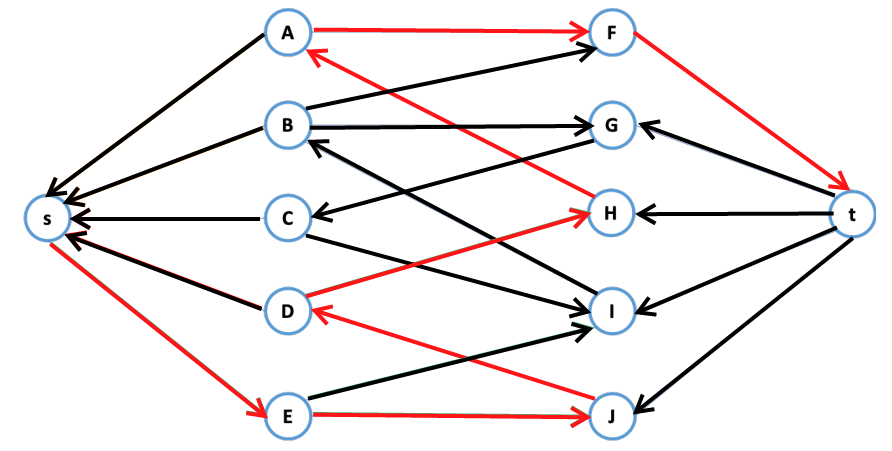
\includegraphics[width=\linewidth]{figures/p4/4.png}
            \caption{Path $P$ connecting $s-t$} 
        \end{figure}

        \begin{figure}[H]
            \centering
            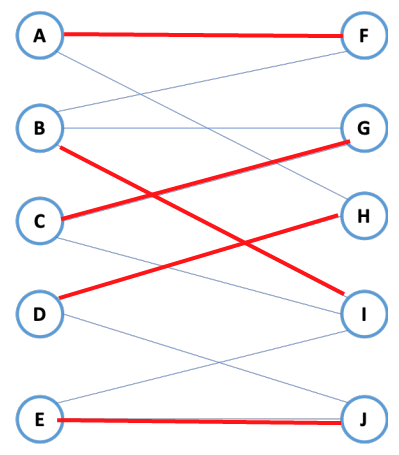
\includegraphics[width=0.4\linewidth]{figures/p4/5.png}
            \caption{Maximum bipartite $M'$} 
        \end{figure}
    \end{tcolorbox}
    \end{enumerate}
\end{section}

\newpage
\begin{section}{Stable Matching}
    There are five companies and five CEO candidates. The companies’ preferences of CEOs are given in the left table below, and the CEOs’ preferences of companies are in the right table.

    \begin{figure}[H]
        \centering
        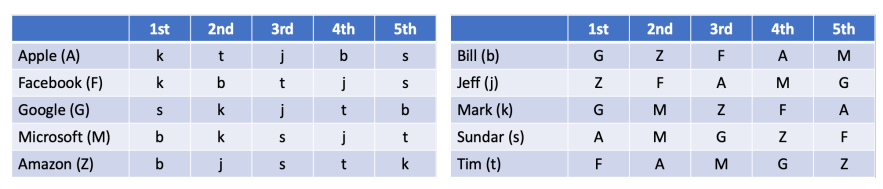
\includegraphics[width=\linewidth]{figures/p5/1.png}
    \end{figure}
    
    \begin{enumerate} [(A)]
        \item Run the Propose-And-Reject Algorithm (Page 9 of lecture note 20 Stable Marriage) based on the companies’ preferences.
        
        \begin{enumerate}[(1)]
            \item Please follow the tutorial problem MM4 Stable Matching. Provide the detailed action and outcome of each step, and highlight the corresponding items in the table.
            
            \begin{tcolorbox}[breakable]
                \begin{enumerate}[(1)]
                    \item $A$ propose to $k$, $k$ is free. So $A-k$
                    \begin{table}[H]
                        \centering
                        \begin{tabular}{|m{2.5cm}|*{5}{c|}}
                            \hline
                            & 1st & 2nd & 3rd & 4th & 5th \\
                            \hline
                            Apple (A)        & {\color{red} k} & t & j & b & s \\
                            Facebook (F)     & k & b & t & j & s \\
                            Google (G)       & s & k & j & t & b \\
                            Microsoft (M)    & b & k & s & j & t \\
                            Amazon (Z)       & b & j & s & t & k \\
                            \hline                            
                        \end{tabular}
                    \end{table}

                    \item $F$ propose to $k$, $k$ is engaged to $A$ but prefers $F$ to $A$ \textrightarrow $A-k$. So $A$ is freed and $F-k$
                    \begin{table}[H]
                        \centering
                        \begin{tabular}{|m{2.5cm}|*{5}{c|}}
                            \hline
                            & 1st & 2nd & 3rd & 4th & 5th \\
                            \hline
                            Apple (A)        & {\color{blue} k} & t & j & b & s \\
                            Facebook (F)     & {\color{red} k} & b & t & j & s \\
                            Google (G)       & s & k & j & t & b \\
                            Microsoft (M)    & b & k & s & j & t \\
                            Amazon (Z)       & b & j & s & t & k \\
                            \hline                            
                        \end{tabular}
                    \end{table}                    

                    \item $A$ propose to $t$, $t$ is free. So $A-t$
                    \begin{table}[H]
                        \centering
                        \begin{tabular}{|m{2.5cm}|*{5}{c|}}
                            \hline
                            & 1st & 2nd & 3rd & 4th & 5th \\
                            \hline
                            Apple (A)        & {\color{blue} k} & {\color{red} t} & j & b & s \\
                            Facebook (F)     & {\color{red} k} & b & t & j & s \\
                            Google (G)       & s & k & j & t & b \\
                            Microsoft (M)    & b & k & s & j & t \\
                            Amazon (Z)       & b & j & s & t & k \\
                            \hline                            
                        \end{tabular}
                    \end{table}                    

                    \item $G$ propose to $s$, $s$ is free. So $G-s$
                    \begin{table}[H]
                        \centering
                        \begin{tabular}{|m{2.5cm}|*{5}{c|}}
                            \hline
                            & 1st & 2nd & 3rd & 4th & 5th \\
                            \hline
                            Apple (A)        & {\color{blue} k} & {\color{red} t} & j & b & s \\
                            Facebook (F)     & {\color{red} k} & b & t & j & s \\
                            Google (G)       & {\color{red} s} & k & j & t & b \\
                            Microsoft (M)    & b & k & s & j & t \\
                            Amazon (Z)       & b & j & s & t & k \\
                            \hline                            
                        \end{tabular}
                    \end{table}                    

                    \item $M$ propose to $b$, $b$ is free. So $M-b$
                    \begin{table}[H]
                        \centering
                        \begin{tabular}{|m{2.5cm}|*{5}{c|}}
                            \hline
                            & 1st & 2nd & 3rd & 4th & 5th \\
                            \hline
                            Apple (A)        & {\color{blue} k} & {\color{red} t} & j & b & s \\
                            Facebook (F)     & {\color{red} k} & b & t & j & s \\
                            Google (G)       & {\color{red} s} & k & j & t & b \\
                            Microsoft (M)    & {\color{red} b} & k & s & j & t \\
                            Amazon (Z)       & b & j & s & t & k \\
                            \hline                            
                        \end{tabular}
                    \end{table}   

                    \item $Z$ propose to $b$, $b$ is engaged to $M$ but prefers $Z$ to $M$. So $M$ is freed and $Z-b$.
                    \begin{table}[H]
                        \centering
                        \begin{tabular}{|m{2.5cm}|*{5}{c|}}
                            \hline
                            & 1st & 2nd & 3rd & 4th & 5th \\
                            \hline
                            Apple (A)        & {\color{blue} k} & {\color{red} t} & j & b & s \\
                            Facebook (F)     & {\color{red} k} & b & t & j & s \\
                            Google (G)       & {\color{red} s} & k & j & t & b \\
                            Microsoft (M)    & {\color{blue} b} & k & s & j & t \\
                            Amazon (Z)       & {\color{red} b} & j & s & t & k \\
                            \hline                            
                        \end{tabular}
                    \end{table}     

                    \item $M$ propose to $k$, $k$ is engaged to $F$ but prefers $M$ to $F$. So $F$ is freed and $M-k$.
                    \begin{table}[H]
                        \centering
                        \begin{tabular}{|m{2.5cm}|*{5}{c|}}
                            \hline
                            & 1st & 2nd & 3rd & 4th & 5th \\
                            \hline
                            Apple (A)        & {\color{blue} k} & {\color{red} t} & j & b & s \\
                            Facebook (F)     & {\color{blue} k} & b & t & j & s \\
                            Google (G)       & {\color{red} s} & k & j & t & b \\
                            Microsoft (M)    & {\color{blue} b} & {\color{red} k} & s & j & t \\
                            Amazon (Z)       & {\color{red} b} & j & s & t & k \\
                            \hline                            
                        \end{tabular}
                    \end{table}                 
                       
                    \item $F$ propose to $b$, $b$ is engaged to $Z$ and prefers $Z$ to $F$. So $F$ is rejected.
                    \begin{table}[H]
                        \centering
                        \begin{tabular}{|m{2.5cm}|*{5}{c|}}
                            \hline
                            & 1st & 2nd & 3rd & 4th & 5th \\
                            \hline
                            Apple (A)        & {\color{blue} k} & {\color{red} t} & j & b & s \\
                            Facebook (F)     & {\color{blue} k} & {\color{blue} b} & t & j & s \\
                            Google (G)       & {\color{red} s} & k & j & t & b \\
                            Microsoft (M)    & {\color{blue} b} & {\color{red} k} & s & j & t \\
                            Amazon (Z)       & {\color{red} b} & j & s & t & k \\
                            \hline                            
                        \end{tabular}
                    \end{table}        

                    \item $F$ propose to $t$, $t$ is engaged to $A$ but prefers $F$ to $A$. So $A$ is freed, $F-t$.
                    \begin{table}[H]
                        \centering
                        \begin{tabular}{|m{2.5cm}|*{5}{c|}}
                            \hline
                            & 1st & 2nd & 3rd & 4th & 5th \\
                            \hline
                            Apple (A)        & {\color{blue} k} & {\color{blue} t} & j & b & s \\
                            Facebook (F)     & {\color{blue} k} & {\color{blue} b} & {\color{red} t} & j & s \\
                            Google (G)       & {\color{red} s} & k & j & t & b \\
                            Microsoft (M)    & {\color{blue} b} & {\color{red} k} & s & j & t \\
                            Amazon (Z)       & {\color{red} b} & j & s & t & k \\
                            \hline                            
                        \end{tabular}
                    \end{table}                    

                    \item $A$ propose to $j$, $j$ is free. So $A-j$.
                    \begin{table}[H]
                        \centering
                        \begin{tabular}{|m{2.5cm}|*{5}{c|}}
                            \hline
                            & 1st & 2nd & 3rd & 4th & 5th \\
                            \hline
                            Apple (A)        & {\color{blue} k} & {\color{blue} t} & {\color{red} j} & b & s \\
                            Facebook (F)     & {\color{blue} k} & {\color{blue} b} & {\color{red} t} & j & s \\
                            Google (G)       & {\color{red} s} & k & j & t & b \\
                            Microsoft (M)    & {\color{blue} b} & {\color{red} k} & s & j & t \\
                            Amazon (Z)       & {\color{red} b} & j & s & t & k \\
                            \hline                            
                        \end{tabular}
                    \end{table}                    
                \end{enumerate}
            \end{tcolorbox}

            \item Provide the final company optimal solution (as a set of matchings.
            \begin{tcolorbox}
                The final matching is $\cbracket{A-j, F-t, G-s, M-k, Z-b}$.
            \end{tcolorbox}

        \end{enumerate}

        \item Run the Propose-And-Reject Algorithm (Page 9 of lecture note 20 Stable Marriage) based on the CEOs’ preferences.
        
        \begin{enumerate}[(1)]
            \item Please follow the tutorial problem MM4 Stable Matching. Provide the detailed action and outcome of each step, and highlight the corresponding items in the table.
            
            \begin{tcolorbox}[breakable]
                \begin{enumerate}[(1)]
                    \item $b$ propose to $G$, $G$ is free. So $b-G$
                    \begin{table}[H]
                        \centering
                        \begin{tabular}{|m{2.5cm}|*{5}{c|}}
                            \hline
                            & 1st & 2nd & 3rd & 4th & 5th \\
                            \hline
                            Bill (b)        & {\color{red} G} & Z & F & A & M \\
                            Jeff (j)        & Z & F & A & M & G \\
                            Mark (k)        & G & M & Z & F & A \\
                            Sundar (s)      & A & M & G & Z & F \\
                            Tim (t)         & F & A & M & G & Z \\
                            \hline                            
                        \end{tabular}
                    \end{table}

                    \item $j$ propose to $Z$, $Z$ is free. So $j-Z$
                    \begin{table}[H]
                        \centering
                        \begin{tabular}{|m{2.5cm}|*{5}{c|}}
                            \hline
                            & 1st & 2nd & 3rd & 4th & 5th \\
                            \hline
                            Bill (b)        & {\color{red} G} & Z & F & A & M \\
                            Jeff (j)        & {\color{red} Z} & F & A & M & G \\
                            Mark (k)        & G & M & Z & F & A \\
                            Sundar (s)      & A & M & G & Z & F \\
                            Tim (t)         & F & A & M & G & Z \\
                            \hline                            
                        \end{tabular}
                    \end{table}

                    \item $k$ propose to $G$, $G$ is engaged to $b$ but prefers $k$ to $b$. So $b$ is freed and $k-G$.
                    \begin{table}[H]
                        \centering
                        \begin{tabular}{|m{2.5cm}|*{5}{c|}}
                            \hline
                            & 1st & 2nd & 3rd & 4th & 5th \\
                            \hline
                            Bill (b)        & {\color{blue} G} & Z & F & A & M \\
                            Jeff (j)        & {\color{red} Z} & F & A & M & G \\
                            Mark (k)        & {\color{red} G} & M & Z & F & A \\
                            Sundar (s)      & A & M & G & Z & F \\
                            Tim (t)         & F & A & M & G & Z \\
                            \hline                            
                        \end{tabular}
                    \end{table}

                    \item $b$ propose to $Z$, $Z$ is engaged to $j$ but prefers $b$ to $j$. So $j$ is freed and $b-Z$.
                    \begin{table}[H]
                        \centering
                        \begin{tabular}{|m{2.5cm}|*{5}{c|}}
                            \hline
                            & 1st & 2nd & 3rd & 4th & 5th \\
                            \hline
                            Bill (b)        & {\color{blue} G} & {\color{red} Z} & F & A & M \\
                            Jeff (j)        & {\color{blue} Z} & F & A & M & G \\
                            Mark (k)        & {\color{red} G} & M & Z & F & A \\
                            Sundar (s)      & A & M & G & Z & F \\
                            Tim (t)         & F & A & M & G & Z \\
                            \hline                            
                        \end{tabular}
                    \end{table}

                    \item $j$ propose to $F$, $F$ is free. So $j-F$.
                    \begin{table}[H]
                        \centering
                        \begin{tabular}{|m{2.5cm}|*{5}{c|}}
                            \hline
                            & 1st & 2nd & 3rd & 4th & 5th \\
                            \hline
                            Bill (b)        & {\color{blue} G} & {\color{red} Z} & F & A & M \\
                            Jeff (j)        & {\color{blue} Z} & {\color{red} F} & A & M & G \\
                            Mark (k)        & {\color{red} G} & M & Z & F & A \\
                            Sundar (s)      & A & M & G & Z & F \\
                            Tim (t)         & F & A & M & G & Z \\
                            \hline                            
                        \end{tabular}
                    \end{table}

                    \item $s$ propose to $A$, $A$ is free. So $s-A$.
                    \begin{table}[H]
                        \centering
                        \begin{tabular}{|m{2.5cm}|*{5}{c|}}
                            \hline
                            & 1st & 2nd & 3rd & 4th & 5th \\
                            \hline
                            Bill (b)        & {\color{blue} G} & {\color{red} Z} & F & A & M \\
                            Jeff (j)        & {\color{blue} Z} & {\color{red} F} & A & M & G \\
                            Mark (k)        & {\color{red} G} & M & Z & F & A \\
                            Sundar (s)      & {\color{red} A} & M & G & Z & F \\
                            Tim (t)         & F & A & M & G & Z \\
                            \hline                            
                        \end{tabular}
                    \end{table}

                    \item $t$ propose to $F$, $F$ is engaged to $j$ but prefers $t$ to $j$. So $j$ is freed and $t-F$.
                    \begin{table}[H]
                        \centering
                        \begin{tabular}{|m{2.5cm}|*{5}{c|}}
                            \hline
                            & 1st & 2nd & 3rd & 4th & 5th \\
                            \hline
                            Bill (b)        & {\color{blue} G} & {\color{red} Z} & F & A & M \\
                            Jeff (j)        & {\color{blue} Z} & {\color{blue} F} & A & M & G \\
                            Mark (k)        & {\color{red} G} & M & Z & F & A \\
                            Sundar (s)      & {\color{red} A} & M & G & Z & F \\
                            Tim (t)         & {\color{red} F} & A & M & G & Z \\
                            \hline                            
                        \end{tabular}
                    \end{table}

                    \item $j$ propose to $A$, $A$ is engaged to $s$ but prefers $j$ to $s$. So $s$ is freed and $j-A$.
                    \begin{table}[H]
                        \centering
                        \begin{tabular}{|m{2.5cm}|*{5}{c|}}
                            \hline
                            & 1st & 2nd & 3rd & 4th & 5th \\
                            \hline
                            Bill (b)        & {\color{blue} G} & {\color{red} Z} & F & A & M \\
                            Jeff (j)        & {\color{blue} Z} & {\color{blue} F} & {\color{red} A} & M & G \\
                            Mark (k)        & {\color{red} G} & M & Z & F & A \\
                            Sundar (s)      & {\color{blue} A} & M & G & Z & F \\
                            Tim (t)         & {\color{red} F} & A & M & G & Z \\
                            \hline                            
                        \end{tabular}
                    \end{table}

                    \item $s$ propose to $M$, $M$ is free. So $s-M$.
                    \begin{table}[H]
                        \centering
                        \begin{tabular}{|m{2.5cm}|*{5}{c|}}
                            \hline
                            & 1st & 2nd & 3rd & 4th & 5th \\
                            \hline
                            Bill (b)        & {\color{blue} G} & {\color{red} Z} & F & A & M \\
                            Jeff (j)        & {\color{blue} Z} & {\color{blue} F} & {\color{red} A} & M & G \\
                            Mark (k)        & {\color{red} G} & M & Z & F & A \\
                            Sundar (s)      & {\color{blue} A} & {\color{red} M} & G & Z & F \\
                            Tim (t)         & {\color{red} F} & A & M & G & Z \\
                            \hline                            
                        \end{tabular}
                    \end{table}

                \end{enumerate}
            \end{tcolorbox}

            \item Provide the final company optimal solution (as a set of matchings.
            \begin{tcolorbox}
                The final matching is $\cbracket{b-Z, j-A, k-G, s-M, t-F}$.
            \end{tcolorbox}
        \end{enumerate}
    \end{enumerate}
\end{section}
\end{document}